\documentclass[1p]{elsarticle_modified}
%\bibliographystyle{elsarticle-num}

%\usepackage[colorlinks]{hyperref}
%\usepackage{abbrmath_seonhwa} %\Abb, \Ascr, \Acal ,\Abf, \Afrak
\usepackage{amsfonts}
\usepackage{amssymb}
\usepackage{amsmath}
\usepackage{amsthm}
\usepackage{scalefnt}
\usepackage{amsbsy}
\usepackage{kotex}
\usepackage{caption}
\usepackage{subfig}
\usepackage{color}
\usepackage{graphicx}
\usepackage{xcolor} %% white, black, red, green, blue, cyan, magenta, yellow
\usepackage{float}
\usepackage{setspace}
\usepackage{hyperref}

\usepackage{tikz}
\usetikzlibrary{arrows}

\usepackage{multirow}
\usepackage{array} % fixed length table
\usepackage{hhline}

%%%%%%%%%%%%%%%%%%%%%
\makeatletter
\renewcommand*\env@matrix[1][\arraystretch]{%
	\edef\arraystretch{#1}%
	\hskip -\arraycolsep
	\let\@ifnextchar\new@ifnextchar
	\array{*\c@MaxMatrixCols c}}
\makeatother %https://tex.stackexchange.com/questions/14071/how-can-i-increase-the-line-spacing-in-a-matrix
%%%%%%%%%%%%%%%

\usepackage[normalem]{ulem}

\newcommand{\msout}[1]{\ifmmode\text{\sout{\ensuremath{#1}}}\else\sout{#1}\fi}
%SOURCE: \msout is \stkout macro in https://tex.stackexchange.com/questions/20609/strikeout-in-math-mode

\newcommand{\cancel}[1]{
	\ifmmode
	{\color{red}\msout{#1}}
	\else
	{\color{red}\sout{#1}}
	\fi
}

\newcommand{\add}[1]{
	{\color{blue}\uwave{#1}}
}

\newcommand{\replace}[2]{
	\ifmmode
	{\color{red}\msout{#1}}{\color{blue}\uwave{#2}}
	\else
	{\color{red}\sout{#1}}{\color{blue}\uwave{#2}}
	\fi
}

\newcommand{\Sol}{\mathcal{S}} %segment
\newcommand{\D}{D} %diagram
\newcommand{\A}{\mathcal{A}} %arc


%%%%%%%%%%%%%%%%%%%%%%%%%%%%%5 test

\def\sl{\operatorname{\textup{SL}}(2,\Cbb)}
\def\psl{\operatorname{\textup{PSL}}(2,\Cbb)}
\def\quan{\mkern 1mu \triangleright \mkern 1mu}

\theoremstyle{definition}
\newtheorem{thm}{Theorem}[section]
\newtheorem{prop}[thm]{Proposition}
\newtheorem{lem}[thm]{Lemma}
\newtheorem{ques}[thm]{Question}
\newtheorem{cor}[thm]{Corollary}
\newtheorem{defn}[thm]{Definition}
\newtheorem{exam}[thm]{Example}
\newtheorem{rmk}[thm]{Remark}
\newtheorem{alg}[thm]{Algorithm}

\newcommand{\I}{\sqrt{-1}}
\begin{document}

%\begin{frontmatter}
%
%\title{Boundary parabolic representations of knots up to 8 crossings}
%
%%% Group authors per affiliation:
%\author{Yunhi Cho} 
%\address{Department of Mathematics, University of Seoul, Seoul, Korea}
%\ead{yhcho@uos.ac.kr}
%
%
%\author{Seonhwa Kim} %\fnref{s_kim}}
%\address{Center for Geometry and Physics, Institute for Basic Science, Pohang, 37673, Korea}
%\ead{ryeona17@ibs.re.kr}
%
%\author{Hyuk Kim}
%\address{Department of Mathematical Sciences, Seoul National University, Seoul 08826, Korea}
%\ead{hyukkim@snu.ac.kr}
%
%\author{Seokbeom Yoon}
%\address{Department of Mathematical Sciences, Seoul National University, Seoul, 08826,  Korea}
%\ead{sbyoon15@snu.ac.kr}
%
%\begin{abstract}
%We find all boundary parabolic representation of knots up to 8 crossings.
%
%\end{abstract}
%\begin{keyword}
%    \MSC[2010] 57M25 
%\end{keyword}
%
%\end{frontmatter}

%\linenumbers
%\tableofcontents
%
\newcommand\colored[1]{\textcolor{white}{\rule[-0.35ex]{0.8em}{1.4ex}}\kern-0.8em\color{red} #1}%
%\newcommand\colored[1]{\textcolor{white}{ #1}\kern-2.17ex	\textcolor{white}{ #1}\kern-1.81ex	\textcolor{white}{ #1}\kern-2.15ex\color{red}#1	}

{\Large $\underline{12a_{0428}~(K12a_{0428})}$}

\setlength{\tabcolsep}{10pt}
\renewcommand{\arraystretch}{1.6}
\vspace{1cm}\begin{tabular}{m{100pt}>{\centering\arraybackslash}m{274pt}}
\multirow{5}{120pt}{
	\centering
	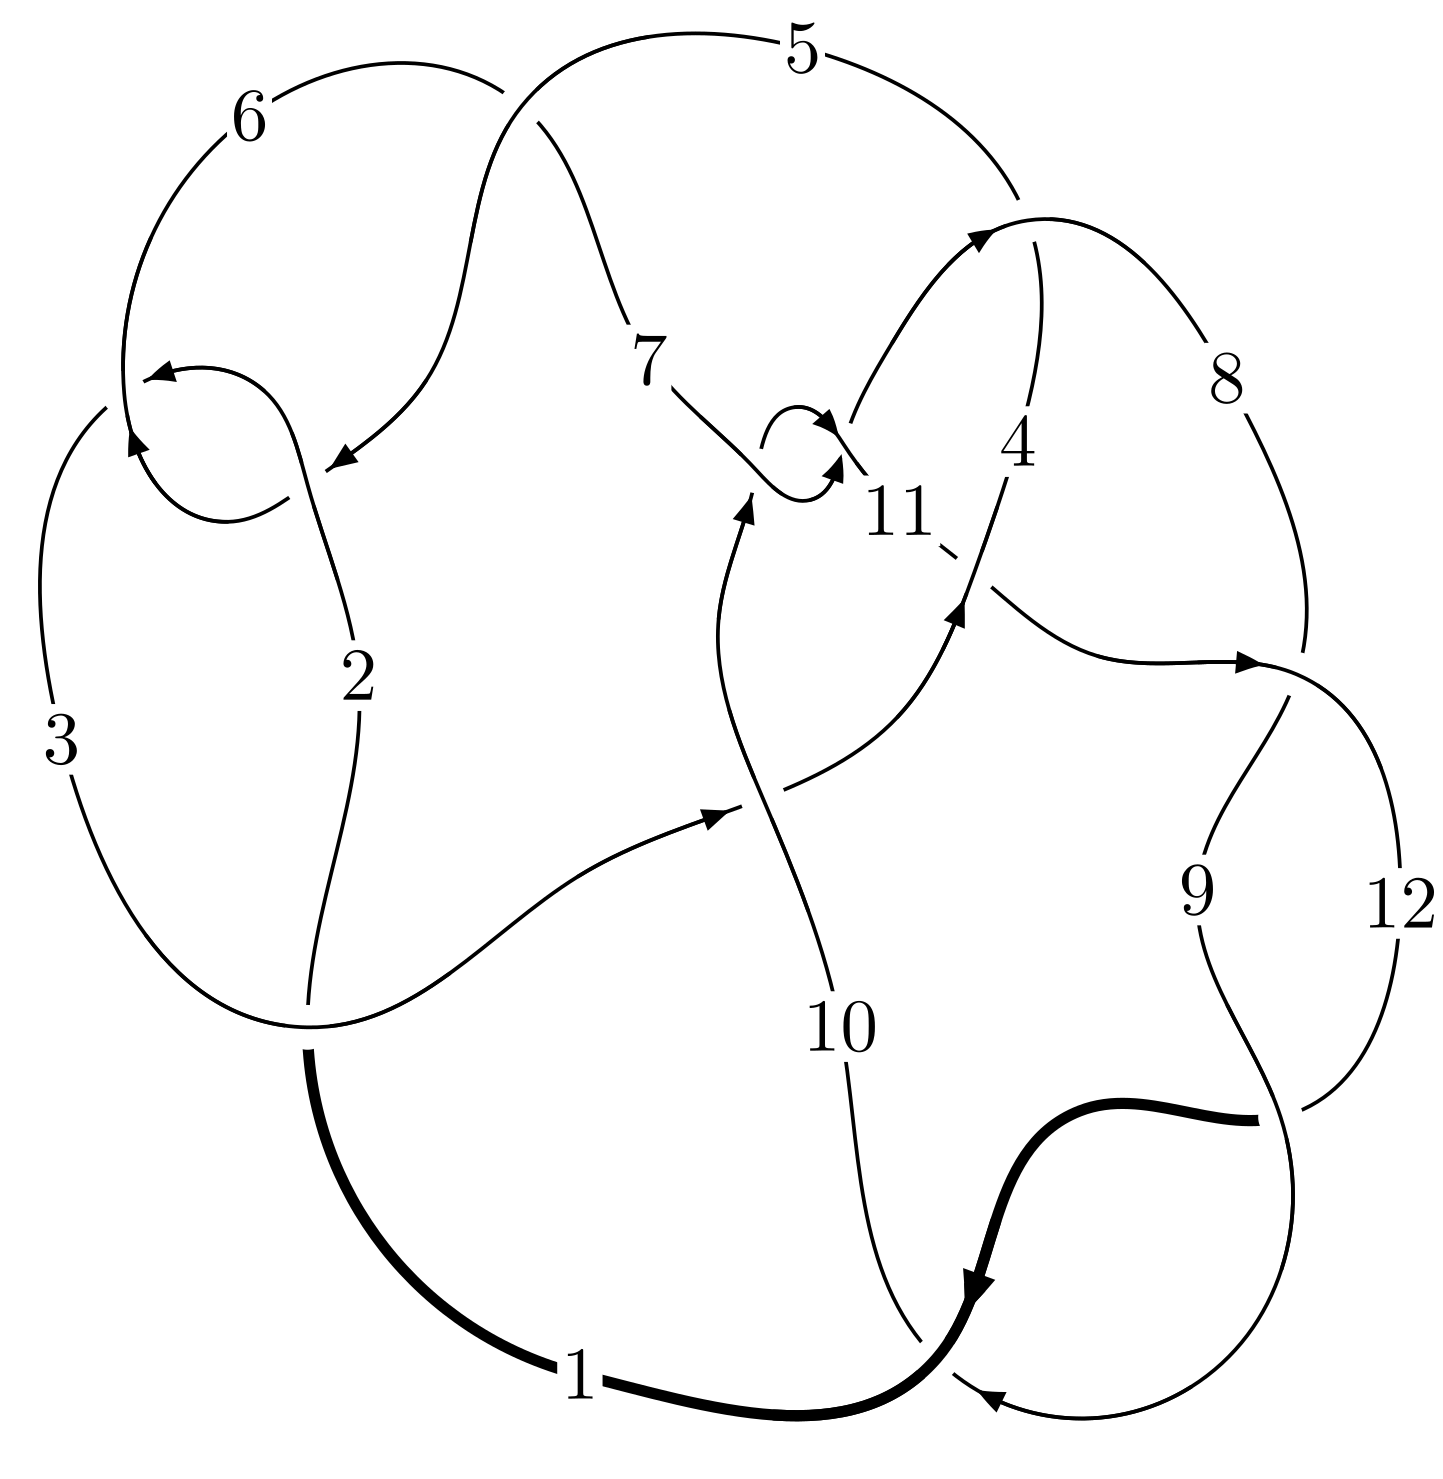
\includegraphics[width=112pt]{../../../GIT/diagram.site/Diagrams/png/1229_12a_0428.png}\\
\ \ \ A knot diagram\footnotemark}&
\allowdisplaybreaks
\textbf{Linearized knot diagam} \\
\cline{2-2}
 &
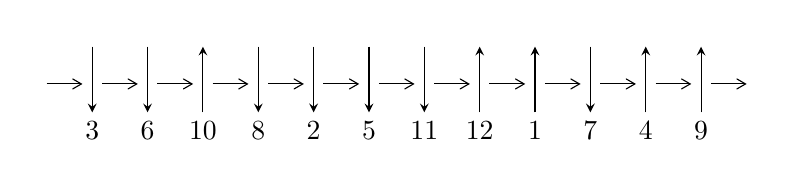
\begin{tikzpicture}[x=20pt, y=17pt]
	% nodes
	\node (C0) at (0, 0) {};
	\node (C1) at (1, 0) {};
	\node (C1U) at (1, +1) {};
	\node (C1D) at (1, -1) {3};

	\node (C2) at (2, 0) {};
	\node (C2U) at (2, +1) {};
	\node (C2D) at (2, -1) {6};

	\node (C3) at (3, 0) {};
	\node (C3U) at (3, +1) {};
	\node (C3D) at (3, -1) {10};

	\node (C4) at (4, 0) {};
	\node (C4U) at (4, +1) {};
	\node (C4D) at (4, -1) {8};

	\node (C5) at (5, 0) {};
	\node (C5U) at (5, +1) {};
	\node (C5D) at (5, -1) {2};

	\node (C6) at (6, 0) {};
	\node (C6U) at (6, +1) {};
	\node (C6D) at (6, -1) {5};

	\node (C7) at (7, 0) {};
	\node (C7U) at (7, +1) {};
	\node (C7D) at (7, -1) {11};

	\node (C8) at (8, 0) {};
	\node (C8U) at (8, +1) {};
	\node (C8D) at (8, -1) {12};

	\node (C9) at (9, 0) {};
	\node (C9U) at (9, +1) {};
	\node (C9D) at (9, -1) {1};

	\node (C10) at (10, 0) {};
	\node (C10U) at (10, +1) {};
	\node (C10D) at (10, -1) {7};

	\node (C11) at (11, 0) {};
	\node (C11U) at (11, +1) {};
	\node (C11D) at (11, -1) {4};

	\node (C12) at (12, 0) {};
	\node (C12U) at (12, +1) {};
	\node (C12D) at (12, -1) {9};
	\node (C13) at (13, 0) {};

	% arrows
	\draw[->,>={angle 60}]
	(C0) edge (C1) (C1) edge (C2) (C2) edge (C3) (C3) edge (C4) (C4) edge (C5) (C5) edge (C6) (C6) edge (C7) (C7) edge (C8) (C8) edge (C9) (C9) edge (C10) (C10) edge (C11) (C11) edge (C12) (C12) edge (C13) ;	\draw[->,>=stealth]
	(C1U) edge (C1D) (C2U) edge (C2D) (C3D) edge (C3U) (C4U) edge (C4D) (C5U) edge (C5D) (C6U) edge (C6D) (C7U) edge (C7D) (C8D) edge (C8U) (C9D) edge (C9U) (C10U) edge (C10D) (C11D) edge (C11U) (C12D) edge (C12U) ;
	\end{tikzpicture} \\
\hhline{~~} \\& 
\textbf{Solving Sequence} \\ \cline{2-2} 
 &
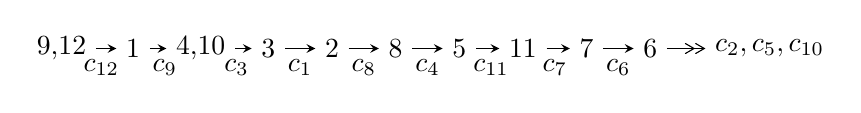
\begin{tikzpicture}[x=23pt, y=7pt]
	% node
	\node (A0) at (-1/8, 0) {9,12};
	\node (A1) at (1, 0) {1};
	\node (A2) at (33/16, 0) {4,10};
	\node (A3) at (25/8, 0) {3};
	\node (A4) at (33/8, 0) {2};
	\node (A5) at (41/8, 0) {8};
	\node (A6) at (49/8, 0) {5};
	\node (A7) at (57/8, 0) {11};
	\node (A8) at (65/8, 0) {7};
	\node (A9) at (73/8, 0) {6};
	\node (C1) at (1/2, -1) {$c_{12}$};
	\node (C2) at (3/2, -1) {$c_{9}$};
	\node (C3) at (21/8, -1) {$c_{3}$};
	\node (C4) at (29/8, -1) {$c_{1}$};
	\node (C5) at (37/8, -1) {$c_{8}$};
	\node (C6) at (45/8, -1) {$c_{4}$};
	\node (C7) at (53/8, -1) {$c_{11}$};
	\node (C8) at (61/8, -1) {$c_{7}$};
	\node (C9) at (69/8, -1) {$c_{6}$};
	\node (A10) at (11, 0) {$c_{2},c_{5},c_{10}$};

	% edge
	\draw[->,>=stealth]	
	(A0) edge (A1) (A1) edge (A2) (A2) edge (A3) (A3) edge (A4) (A4) edge (A5) (A5) edge (A6) (A6) edge (A7) (A7) edge (A8) (A8) edge (A9) ;
	\draw[->>,>={angle 60}]	
	(A9) edge (A10);
\end{tikzpicture} \\ 

\end{tabular} \\

\footnotetext{
The image of knot diagram is generated by the software ``\textbf{Draw programme}" developed by Andrew Bartholomew(\url{http://www.layer8.co.uk/maths/draw/index.htm\#Running-draw}), where we modified some parts for our purpose(\url{https://github.com/CATsTAILs/LinksPainter}).
}\phantom \\ \newline 
\centering \textbf{Ideals for irreducible components\footnotemark of $X_{\text{par}}$} 
 
\begin{align*}
I^u_{1}&=\langle 
2.80676\times10^{126} u^{84}-1.58226\times10^{127} u^{83}+\cdots+6.30962\times10^{126} b-8.39340\times10^{126},\\
\phantom{I^u_{1}}&\phantom{= \langle  }-8.84774\times10^{126} u^{84}+5.87857\times10^{127} u^{83}+\cdots+6.30962\times10^{126} a+7.56669\times10^{127},\\
\phantom{I^u_{1}}&\phantom{= \langle  }u^{85}-7 u^{84}+\cdots-6 u+2\rangle \\
I^u_{2}&=\langle 
b+1,\;2 a+u-4,\;u^2-2\rangle \\
\\
I^v_{1}&=\langle 
a,\;b-1,\;v-1\rangle \\
\end{align*}
\raggedright * 3 irreducible components of $\dim_{\mathbb{C}}=0$, with total 88 representations.\\
\footnotetext{All coefficients of polynomials are rational numbers. But the coefficients are sometimes approximated in decimal forms when there is not enough margin.}
\newpage
\renewcommand{\arraystretch}{1}
\centering \section*{I. $I^u_{1}= \langle 2.81\times10^{126} u^{84}-1.58\times10^{127} u^{83}+\cdots+6.31\times10^{126} b-8.39\times10^{126},\;-8.85\times10^{126} u^{84}+5.88\times10^{127} u^{83}+\cdots+6.31\times10^{126} a+7.57\times10^{127},\;u^{85}-7 u^{84}+\cdots-6 u+2 \rangle$}
\flushleft \textbf{(i) Arc colorings}\\
\begin{tabular}{m{7pt} m{180pt} m{7pt} m{180pt} }
\flushright $a_{9}=$&$\begin{pmatrix}0\\u\end{pmatrix}$ \\
\flushright $a_{12}=$&$\begin{pmatrix}1\\0\end{pmatrix}$ \\
\flushright $a_{1}=$&$\begin{pmatrix}1\\- u^2\end{pmatrix}$ \\
\flushright $a_{4}=$&$\begin{pmatrix}1.40226 u^{84}-9.31684 u^{83}+\cdots-23.5188 u-11.9923\\-0.444839 u^{84}+2.50770 u^{83}+\cdots-0.499951 u+1.33025\end{pmatrix}$ \\
\flushright $a_{10}=$&$\begin{pmatrix}u\\- u^3+u\end{pmatrix}$ \\
\flushright $a_{3}=$&$\begin{pmatrix}1.47259 u^{84}-9.46618 u^{83}+\cdots-22.8706 u-13.0462\\-0.418554 u^{84}+2.03469 u^{83}+\cdots-1.76897 u+0.962317\end{pmatrix}$ \\
\flushright $a_{2}=$&$\begin{pmatrix}-1.84257 u^{84}+11.7840 u^{83}+\cdots+18.6397 u+10.0949\\1.51198 u^{84}-8.84490 u^{83}+\cdots+3.89018 u-2.11365\end{pmatrix}$ \\
\flushright $a_{8}=$&$\begin{pmatrix}- u\\u\end{pmatrix}$ \\
\flushright $a_{5}=$&$\begin{pmatrix}1.67889 u^{84}-10.4912 u^{83}+\cdots-20.9610 u-12.2067\\-0.721468 u^{84}+3.68203 u^{83}+\cdots-3.05782 u+1.54459\end{pmatrix}$ \\
\flushright $a_{11}=$&$\begin{pmatrix}0.138261 u^{84}-1.44715 u^{83}+\cdots-8.35732 u-4.42866\\0.360457 u^{84}-2.01792 u^{83}+\cdots+1.41000 u-0.981112\end{pmatrix}$ \\
\flushright $a_{7}=$&$\begin{pmatrix}-0.138261 u^{84}+1.44715 u^{83}+\cdots+8.35732 u+4.42866\\-0.519401 u^{84}+2.66327 u^{83}+\cdots-1.74245 u-0.0224697\end{pmatrix}$ \\
\flushright $a_{6}=$&$\begin{pmatrix}1.22347 u^{84}-7.56601 u^{83}+\cdots-9.48559 u-3.57665\\-1.38509 u^{84}+7.99231 u^{83}+\cdots-3.90685 u+1.41003\end{pmatrix}$\\&\end{tabular}
\flushleft \textbf{(ii) Obstruction class $= -1$}\\~\\
\flushleft \textbf{(iii) Cusp Shapes $= -4.04066 u^{84}+28.4088 u^{83}+\cdots+78.3664 u+30.4352$}\\~\\
\newpage\renewcommand{\arraystretch}{1}
\flushleft \textbf{(iv) u-Polynomials at the component}\newline \\
\begin{tabular}{m{50pt}|m{274pt}}
Crossings & \hspace{64pt}u-Polynomials at each crossing \\
\hline $$\begin{aligned}c_{1},c_{6}\end{aligned}$$&$\begin{aligned}
&u^{85}+26 u^{84}+\cdots+138 u+1
\end{aligned}$\\
\hline $$\begin{aligned}c_{2},c_{5}\end{aligned}$$&$\begin{aligned}
&u^{85}+4 u^{84}+\cdots-10 u+1
\end{aligned}$\\
\hline $$\begin{aligned}c_{3}\end{aligned}$$&$\begin{aligned}
&u^{85}-30 u^{84}+\cdots+3982062 u+182711
\end{aligned}$\\
\hline $$\begin{aligned}c_{4}\end{aligned}$$&$\begin{aligned}
&u^{85}+24 u^{84}+\cdots+38 u+349
\end{aligned}$\\
\hline $$\begin{aligned}c_{7},c_{10}\end{aligned}$$&$\begin{aligned}
&u^{85}+2 u^{84}+\cdots+22 u+1
\end{aligned}$\\
\hline $$\begin{aligned}c_{8},c_{9},c_{12}\end{aligned}$$&$\begin{aligned}
&u^{85}-7 u^{84}+\cdots-6 u+2
\end{aligned}$\\
\hline $$\begin{aligned}c_{11}\end{aligned}$$&$\begin{aligned}
&u^{85}-4 u^{84}+\cdots-10 u+1
\end{aligned}$\\
\hline
\end{tabular}\\~\\
\newpage\renewcommand{\arraystretch}{1}
\flushleft \textbf{(v) Riley Polynomials at the component}\newline \\
\begin{tabular}{m{50pt}|m{274pt}}
Crossings & \hspace{64pt}Riley Polynomials at each crossing \\
\hline $$\begin{aligned}c_{1},c_{6}\end{aligned}$$&$\begin{aligned}
&y^{85}+70 y^{84}+\cdots+18106 y-1
\end{aligned}$\\
\hline $$\begin{aligned}c_{2},c_{5}\end{aligned}$$&$\begin{aligned}
&y^{85}-26 y^{84}+\cdots+138 y-1
\end{aligned}$\\
\hline $$\begin{aligned}c_{3}\end{aligned}$$&$\begin{aligned}
&y^{85}-266 y^{84}+\cdots+5409686724738 y-33383309521
\end{aligned}$\\
\hline $$\begin{aligned}c_{4}\end{aligned}$$&$\begin{aligned}
&y^{85}-258 y^{84}+\cdots-3360822 y-121801
\end{aligned}$\\
\hline $$\begin{aligned}c_{7},c_{10}\end{aligned}$$&$\begin{aligned}
&y^{85}-50 y^{84}+\cdots+210 y-1
\end{aligned}$\\
\hline $$\begin{aligned}c_{8},c_{9},c_{12}\end{aligned}$$&$\begin{aligned}
&y^{85}-91 y^{84}+\cdots+84 y-4
\end{aligned}$\\
\hline $$\begin{aligned}c_{11}\end{aligned}$$&$\begin{aligned}
&y^{85}-10 y^{84}+\cdots+82 y-1
\end{aligned}$\\
\hline
\end{tabular}\\~\\
\newpage\flushleft \textbf{(vi) Complex Volumes and Cusp Shapes}
$$\begin{array}{c|c|c}  
\text{Solutions to }I^u_{1}& \I (\text{vol} + \sqrt{-1}CS) & \text{Cusp shape}\\
 \hline 
\begin{aligned}
u &= -0.350398 + 0.954037 I \\
a &= -0.219916 + 0.109779 I \\
b &= -0.615170 - 0.648027 I\end{aligned}
 & \phantom{-}1.23620 + 1.62017 I & \phantom{-0.000000 } 0 \\ \hline\begin{aligned}
u &= -0.350398 - 0.954037 I \\
a &= -0.219916 - 0.109779 I \\
b &= -0.615170 + 0.648027 I\end{aligned}
 & \phantom{-}1.23620 - 1.62017 I & \phantom{-0.000000 } 0 \\ \hline\begin{aligned}
u &= -0.689400 + 0.747068 I \\
a &= -0.820189 - 0.472975 I \\
b &= \phantom{-}0.887204 - 0.981521 I\end{aligned}
 & \phantom{-}2.30710 - 7.08904 I & \phantom{-0.000000 } 0 \\ \hline\begin{aligned}
u &= -0.689400 - 0.747068 I \\
a &= -0.820189 + 0.472975 I \\
b &= \phantom{-}0.887204 + 0.981521 I\end{aligned}
 & \phantom{-}2.30710 + 7.08904 I & \phantom{-0.000000 } 0 \\ \hline\begin{aligned}
u &= -0.663371 + 0.802333 I \\
a &= \phantom{-}0.809381 + 0.448944 I \\
b &= -0.903277 + 0.986202 I\end{aligned}
 & \phantom{-}1.47284 - 13.12350 I & \phantom{-0.000000 } 0 \\ \hline\begin{aligned}
u &= -0.663371 - 0.802333 I \\
a &= \phantom{-}0.809381 - 0.448944 I \\
b &= -0.903277 - 0.986202 I\end{aligned}
 & \phantom{-}1.47284 + 13.12350 I & \phantom{-0.000000 } 0 \\ \hline\begin{aligned}
u &= -0.443639 + 0.971475 I \\
a &= \phantom{-}0.188178 - 0.202759 I \\
b &= \phantom{-}0.625699 + 0.679357 I\end{aligned}
 & \phantom{-}0.74636 + 7.39297 I & \phantom{-0.000000 } 0 \\ \hline\begin{aligned}
u &= -0.443639 - 0.971475 I \\
a &= \phantom{-}0.188178 + 0.202759 I \\
b &= \phantom{-}0.625699 - 0.679357 I\end{aligned}
 & \phantom{-}0.74636 - 7.39297 I & \phantom{-0.000000 } 0 \\ \hline\begin{aligned}
u &= -0.582158 + 0.684632 I \\
a &= \phantom{-}0.424934 - 0.552027 I \\
b &= \phantom{-}0.520307 + 0.764862 I\end{aligned}
 & -4.75882 + 3.00452 I & \phantom{-0.000000 } 0 \\ \hline\begin{aligned}
u &= -0.582158 - 0.684632 I \\
a &= \phantom{-}0.424934 + 0.552027 I \\
b &= \phantom{-}0.520307 - 0.764862 I\end{aligned}
 & -4.75882 - 3.00452 I & \phantom{-0.000000 } 0\\
 \hline 
 \end{array}$$\newpage$$\begin{array}{c|c|c}  
\text{Solutions to }I^u_{1}& \I (\text{vol} + \sqrt{-1}CS) & \text{Cusp shape}\\
 \hline 
\begin{aligned}
u &= -0.483276 + 0.686746 I \\
a &= \phantom{-}0.721089 + 0.479217 I \\
b &= -0.894296 + 1.050870 I\end{aligned}
 & -5.01547 - 7.61885 I & \phantom{-0.000000 } 0 \\ \hline\begin{aligned}
u &= -0.483276 - 0.686746 I \\
a &= \phantom{-}0.721089 - 0.479217 I \\
b &= -0.894296 - 1.050870 I\end{aligned}
 & -5.01547 + 7.61885 I & \phantom{-0.000000 } 0 \\ \hline\begin{aligned}
u &= -0.780126 + 0.247893 I \\
a &= \phantom{-}0.24627 - 1.42990 I \\
b &= \phantom{-}0.260947 + 0.994313 I\end{aligned}
 & -3.10853 - 1.92390 I & \phantom{-0.000000 } 0 \\ \hline\begin{aligned}
u &= -0.780126 - 0.247893 I \\
a &= \phantom{-}0.24627 + 1.42990 I \\
b &= \phantom{-}0.260947 - 0.994313 I\end{aligned}
 & -3.10853 + 1.92390 I & \phantom{-0.000000 } 0 \\ \hline\begin{aligned}
u &= \phantom{-}0.352197 + 0.734345 I \\
a &= \phantom{-}0.228751 - 0.454302 I \\
b &= -0.622349 - 0.427633 I\end{aligned}
 & -0.61148 + 3.02035 I & \phantom{-0.000000 } 0 \\ \hline\begin{aligned}
u &= \phantom{-}0.352197 - 0.734345 I \\
a &= \phantom{-}0.228751 + 0.454302 I \\
b &= -0.622349 + 0.427633 I\end{aligned}
 & -0.61148 - 3.02035 I & \phantom{-0.000000 } 0 \\ \hline\begin{aligned}
u &= \phantom{-}0.718711 + 0.953380 I \\
a &= \phantom{-}0.334403 - 0.245488 I \\
b &= -0.690642 - 0.403366 I\end{aligned}
 & \phantom{-}5.16840 + 6.32915 I & \phantom{-0.000000 } 0 \\ \hline\begin{aligned}
u &= \phantom{-}0.718711 - 0.953380 I \\
a &= \phantom{-}0.334403 + 0.245488 I \\
b &= -0.690642 + 0.403366 I\end{aligned}
 & \phantom{-}5.16840 - 6.32915 I & \phantom{-0.000000 } 0 \\ \hline\begin{aligned}
u &= \phantom{-}0.797687 + 0.893769 I \\
a &= -0.365741 + 0.245017 I \\
b &= \phantom{-}0.687642 + 0.390239 I\end{aligned}
 & \phantom{-}5.44394 + 0.44289 I & \phantom{-0.000000 } 0 \\ \hline\begin{aligned}
u &= \phantom{-}0.797687 - 0.893769 I \\
a &= -0.365741 - 0.245017 I \\
b &= \phantom{-}0.687642 - 0.390239 I\end{aligned}
 & \phantom{-}5.44394 - 0.44289 I & \phantom{-0.000000 } 0\\
 \hline 
 \end{array}$$\newpage$$\begin{array}{c|c|c}  
\text{Solutions to }I^u_{1}& \I (\text{vol} + \sqrt{-1}CS) & \text{Cusp shape}\\
 \hline 
\begin{aligned}
u &= -0.523520 + 0.498463 I \\
a &= -0.694604 - 0.589082 I \\
b &= \phantom{-}0.805309 - 1.079360 I\end{aligned}
 & -1.28750 - 4.47163 I & \phantom{-0.000000 -}0. + 7.27748 I \\ \hline\begin{aligned}
u &= -0.523520 - 0.498463 I \\
a &= -0.694604 + 0.589082 I \\
b &= \phantom{-}0.805309 + 1.079360 I\end{aligned}
 & -1.28750 + 4.47163 I & \phantom{-0.000000 } 0. - 7.27748 I \\ \hline\begin{aligned}
u &= \phantom{-}1.312140 + 0.034317 I \\
a &= -0.288123 - 0.083227 I \\
b &= \phantom{-}0.282890 - 0.765202 I\end{aligned}
 & \phantom{-}2.85614 + 1.44672 I & \phantom{-0.000000 } 0 \\ \hline\begin{aligned}
u &= \phantom{-}1.312140 - 0.034317 I \\
a &= -0.288123 + 0.083227 I \\
b &= \phantom{-}0.282890 + 0.765202 I\end{aligned}
 & \phantom{-}2.85614 - 1.44672 I & \phantom{-0.000000 } 0 \\ \hline\begin{aligned}
u &= \phantom{-}0.633148 + 0.261587 I \\
a &= -0.599636 - 0.162415 I \\
b &= \phantom{-}1.010410 - 0.616700 I\end{aligned}
 & \phantom{-}3.19350 + 0.56226 I & \phantom{-}3.06377 - 2.90425 I \\ \hline\begin{aligned}
u &= \phantom{-}0.633148 - 0.261587 I \\
a &= -0.599636 + 0.162415 I \\
b &= \phantom{-}1.010410 + 0.616700 I\end{aligned}
 & \phantom{-}3.19350 - 0.56226 I & \phantom{-}3.06377 + 2.90425 I \\ \hline\begin{aligned}
u &= \phantom{-}0.540521 + 0.360690 I \\
a &= \phantom{-}0.590908 + 0.173669 I \\
b &= -1.095800 + 0.703881 I\end{aligned}
 & \phantom{-}2.25501 + 6.33839 I & \phantom{-}0.16573 - 8.82951 I \\ \hline\begin{aligned}
u &= \phantom{-}0.540521 - 0.360690 I \\
a &= \phantom{-}0.590908 - 0.173669 I \\
b &= -1.095800 - 0.703881 I\end{aligned}
 & \phantom{-}2.25501 - 6.33839 I & \phantom{-}0.16573 + 8.82951 I \\ \hline\begin{aligned}
u &= \phantom{-}0.550804 + 0.330376 I \\
a &= -0.605955 + 0.401645 I \\
b &= \phantom{-}0.664924 + 0.336752 I\end{aligned}
 & \phantom{-}1.141080 + 0.674467 I & \phantom{-}6.05979 - 2.03685 I \\ \hline\begin{aligned}
u &= \phantom{-}0.550804 - 0.330376 I \\
a &= -0.605955 - 0.401645 I \\
b &= \phantom{-}0.664924 - 0.336752 I\end{aligned}
 & \phantom{-}1.141080 - 0.674467 I & \phantom{-}6.05979 + 2.03685 I\\
 \hline 
 \end{array}$$\newpage$$\begin{array}{c|c|c}  
\text{Solutions to }I^u_{1}& \I (\text{vol} + \sqrt{-1}CS) & \text{Cusp shape}\\
 \hline 
\begin{aligned}
u &= \phantom{-}1.373900 + 0.312502 I \\
a &= -0.546242 + 0.208542 I \\
b &= \phantom{-}0.540012 + 0.290386 I\end{aligned}
 & \phantom{-}2.32626 + 1.44371 I & \phantom{-0.000000 } 0 \\ \hline\begin{aligned}
u &= \phantom{-}1.373900 - 0.312502 I \\
a &= -0.546242 - 0.208542 I \\
b &= \phantom{-}0.540012 - 0.290386 I\end{aligned}
 & \phantom{-}2.32626 - 1.44371 I & \phantom{-0.000000 } 0 \\ \hline\begin{aligned}
u &= -1.40914\phantom{ +0.000000I} \\
a &= -16.7791\phantom{ +0.000000I} \\
b &= \phantom{-}0.101896\phantom{ +0.000000I}\end{aligned}
 & \phantom{-}2.16646\phantom{ +0.000000I} & \phantom{-0.000000 } 0 \\ \hline\begin{aligned}
u &= -0.575916 + 0.039342 I \\
a &= -0.56776 + 1.38481 I \\
b &= \phantom{-}0.314595 + 0.853851 I\end{aligned}
 & \phantom{-}4.04443 + 2.89490 I & \phantom{-}2.62420 - 5.69184 I \\ \hline\begin{aligned}
u &= -0.575916 - 0.039342 I \\
a &= -0.56776 - 1.38481 I \\
b &= \phantom{-}0.314595 - 0.853851 I\end{aligned}
 & \phantom{-}4.04443 - 2.89490 I & \phantom{-}2.62420 + 5.69184 I \\ \hline\begin{aligned}
u &= -1.42933\phantom{ +0.000000I} \\
a &= -2.01148\phantom{ +0.000000I} \\
b &= \phantom{-}1.27671\phantom{ +0.000000I}\end{aligned}
 & \phantom{-}3.31731\phantom{ +0.000000I} & \phantom{-0.000000 } 0 \\ \hline\begin{aligned}
u &= -1.43615 + 0.00633 I \\
a &= -1.07681 + 8.24758 I \\
b &= \phantom{-}0.026127 + 0.202391 I\end{aligned}
 & \phantom{-}6.35829 - 2.84127 I & \phantom{-0.000000 } 0 \\ \hline\begin{aligned}
u &= -1.43615 - 0.00633 I \\
a &= -1.07681 - 8.24758 I \\
b &= \phantom{-}0.026127 - 0.202391 I\end{aligned}
 & \phantom{-}6.35829 + 2.84127 I & \phantom{-0.000000 } 0 \\ \hline\begin{aligned}
u &= -0.302575 + 0.455380 I \\
a &= -1.49220 + 0.23122 I \\
b &= -0.383548 - 0.612585 I\end{aligned}
 & -1.80646 + 1.16535 I & -2.20309 + 0.49603 I \\ \hline\begin{aligned}
u &= -0.302575 - 0.455380 I \\
a &= -1.49220 - 0.23122 I \\
b &= -0.383548 + 0.612585 I\end{aligned}
 & -1.80646 - 1.16535 I & -2.20309 - 0.49603 I\\
 \hline 
 \end{array}$$\newpage$$\begin{array}{c|c|c}  
\text{Solutions to }I^u_{1}& \I (\text{vol} + \sqrt{-1}CS) & \text{Cusp shape}\\
 \hline 
\begin{aligned}
u &= \phantom{-}1.46581\phantom{ +0.000000I} \\
a &= \phantom{-}1.07213\phantom{ +0.000000I} \\
b &= -0.291522\phantom{ +0.000000I}\end{aligned}
 & \phantom{-}3.38907\phantom{ +0.000000I} & \phantom{-0.000000 } 0 \\ \hline\begin{aligned}
u &= \phantom{-}1.47026 + 0.09843 I \\
a &= -1.90184 - 1.00109 I \\
b &= \phantom{-}1.48075 + 1.64599 I\end{aligned}
 & \phantom{-}1.40995 + 2.41389 I & \phantom{-0.000000 } 0 \\ \hline\begin{aligned}
u &= \phantom{-}1.47026 - 0.09843 I \\
a &= -1.90184 + 1.00109 I \\
b &= \phantom{-}1.48075 - 1.64599 I\end{aligned}
 & \phantom{-}1.40995 - 2.41389 I & \phantom{-0.000000 } 0 \\ \hline\begin{aligned}
u &= -0.301501 + 0.430647 I \\
a &= \phantom{-}0.540764 + 0.519219 I \\
b &= -0.87964 + 1.24285 I\end{aligned}
 & -4.44895 - 0.68347 I & -8.48630 + 5.94537 I \\ \hline\begin{aligned}
u &= -0.301501 - 0.430647 I \\
a &= \phantom{-}0.540764 - 0.519219 I \\
b &= -0.87964 - 1.24285 I\end{aligned}
 & -4.44895 + 0.68347 I & -8.48630 - 5.94537 I \\ \hline\begin{aligned}
u &= -1.47467\phantom{ +0.000000I} \\
a &= -2.37463\phantom{ +0.000000I} \\
b &= \phantom{-}2.10239\phantom{ +0.000000I}\end{aligned}
 & \phantom{-}3.16776\phantom{ +0.000000I} & \phantom{-0.000000 } 0 \\ \hline\begin{aligned}
u &= -0.498452 + 0.140002 I \\
a &= \phantom{-}0.54620 - 1.67577 I \\
b &= -0.250598 - 0.735061 I\end{aligned}
 & \phantom{-}3.84985 - 3.08699 I & \phantom{-}1.200909 + 0.416894 I \\ \hline\begin{aligned}
u &= -0.498452 - 0.140002 I \\
a &= \phantom{-}0.54620 + 1.67577 I \\
b &= -0.250598 + 0.735061 I\end{aligned}
 & \phantom{-}3.84985 + 3.08699 I & \phantom{-}1.200909 - 0.416894 I \\ \hline\begin{aligned}
u &= -1.46964 + 0.20672 I \\
a &= -1.54329 - 0.13102 I \\
b &= \phantom{-}1.099320 - 0.617535 I\end{aligned}
 & \phantom{-}5.32596 - 6.27686 I & \phantom{-0.000000 } 0 \\ \hline\begin{aligned}
u &= -1.46964 - 0.20672 I \\
a &= -1.54329 + 0.13102 I \\
b &= \phantom{-}1.099320 + 0.617535 I\end{aligned}
 & \phantom{-}5.32596 + 6.27686 I & \phantom{-0.000000 } 0\\
 \hline 
 \end{array}$$\newpage$$\begin{array}{c|c|c}  
\text{Solutions to }I^u_{1}& \I (\text{vol} + \sqrt{-1}CS) & \text{Cusp shape}\\
 \hline 
\begin{aligned}
u &= \phantom{-}1.50742 + 0.21678 I \\
a &= -1.88143 - 0.35406 I \\
b &= \phantom{-}1.30541 + 1.20213 I\end{aligned}
 & \phantom{-}1.48847 + 10.87230 I & \phantom{-0.000000 } 0 \\ \hline\begin{aligned}
u &= \phantom{-}1.50742 - 0.21678 I \\
a &= -1.88143 + 0.35406 I \\
b &= \phantom{-}1.30541 - 1.20213 I\end{aligned}
 & \phantom{-}1.48847 - 10.87230 I & \phantom{-0.000000 } 0 \\ \hline\begin{aligned}
u &= \phantom{-}1.52560 + 0.04894 I \\
a &= -0.732565 + 0.568243 I \\
b &= \phantom{-}0.60909 - 1.42456 I\end{aligned}
 & \phantom{-}10.66790 + 3.82825 I & \phantom{-0.000000 } 0 \\ \hline\begin{aligned}
u &= \phantom{-}1.52560 - 0.04894 I \\
a &= -0.732565 - 0.568243 I \\
b &= \phantom{-}0.60909 + 1.42456 I\end{aligned}
 & \phantom{-}10.66790 - 3.82825 I & \phantom{-0.000000 } 0 \\ \hline\begin{aligned}
u &= -1.52356 + 0.11089 I \\
a &= \phantom{-}1.64270 - 0.07825 I \\
b &= -1.262990 + 0.607994 I\end{aligned}
 & \phantom{-}7.99831 - 2.36928 I & \phantom{-0.000000 } 0 \\ \hline\begin{aligned}
u &= -1.52356 - 0.11089 I \\
a &= \phantom{-}1.64270 + 0.07825 I \\
b &= -1.262990 - 0.607994 I\end{aligned}
 & \phantom{-}7.99831 + 2.36928 I & \phantom{-0.000000 } 0 \\ \hline\begin{aligned}
u &= -1.53057 + 0.09366 I \\
a &= -1.58412 - 0.90265 I \\
b &= \phantom{-}1.53360 + 1.16611 I\end{aligned}
 & \phantom{-}9.16879 - 7.92620 I & \phantom{-0.000000 } 0 \\ \hline\begin{aligned}
u &= -1.53057 - 0.09366 I \\
a &= -1.58412 + 0.90265 I \\
b &= \phantom{-}1.53360 - 1.16611 I\end{aligned}
 & \phantom{-}9.16879 + 7.92620 I & \phantom{-0.000000 } 0 \\ \hline\begin{aligned}
u &= \phantom{-}1.52747 + 0.14748 I \\
a &= \phantom{-}1.72231 + 0.56923 I \\
b &= -1.26106 - 1.37468 I\end{aligned}
 & \phantom{-}5.52175 + 6.80206 I & \phantom{-0.000000 } 0 \\ \hline\begin{aligned}
u &= \phantom{-}1.52747 - 0.14748 I \\
a &= \phantom{-}1.72231 - 0.56923 I \\
b &= -1.26106 + 1.37468 I\end{aligned}
 & \phantom{-}5.52175 - 6.80206 I & \phantom{-0.000000 } 0\\
 \hline 
 \end{array}$$\newpage$$\begin{array}{c|c|c}  
\text{Solutions to }I^u_{1}& \I (\text{vol} + \sqrt{-1}CS) & \text{Cusp shape}\\
 \hline 
\begin{aligned}
u &= \phantom{-}1.54188 + 0.01197 I \\
a &= \phantom{-}0.905976 - 0.683222 I \\
b &= -0.73000 + 1.51724 I\end{aligned}
 & \phantom{-}11.17630 - 2.69311 I & \phantom{-0.000000 } 0 \\ \hline\begin{aligned}
u &= \phantom{-}1.54188 - 0.01197 I \\
a &= \phantom{-}0.905976 + 0.683222 I \\
b &= -0.73000 - 1.51724 I\end{aligned}
 & \phantom{-}11.17630 + 2.69311 I & \phantom{-0.000000 } 0 \\ \hline\begin{aligned}
u &= \phantom{-}0.217769 + 0.395625 I \\
a &= -2.31457 + 3.78349 I \\
b &= \phantom{-}0.549464 + 0.358418 I\end{aligned}
 & \phantom{-}1.33766 - 3.69180 I & -2.91564 - 6.56746 I \\ \hline\begin{aligned}
u &= \phantom{-}0.217769 - 0.395625 I \\
a &= -2.31457 - 3.78349 I \\
b &= \phantom{-}0.549464 - 0.358418 I\end{aligned}
 & \phantom{-}1.33766 + 3.69180 I & -2.91564 + 6.56746 I \\ \hline\begin{aligned}
u &= \phantom{-}0.137119 + 0.429179 I \\
a &= \phantom{-}1.41458 - 3.63175 I \\
b &= -0.508025 - 0.397814 I\end{aligned}
 & \phantom{-}1.61743 + 1.92054 I & -4.53145 - 10.20212 I \\ \hline\begin{aligned}
u &= \phantom{-}0.137119 - 0.429179 I \\
a &= \phantom{-}1.41458 + 3.63175 I \\
b &= -0.508025 + 0.397814 I\end{aligned}
 & \phantom{-}1.61743 - 1.92054 I & -4.53145 + 10.20212 I \\ \hline\begin{aligned}
u &= -1.55025 + 0.05271 I \\
a &= \phantom{-}1.65971 + 0.68673 I \\
b &= -1.54955 - 0.98630 I\end{aligned}
 & \phantom{-}10.50810 - 1.58318 I & \phantom{-0.000000 } 0 \\ \hline\begin{aligned}
u &= -1.55025 - 0.05271 I \\
a &= \phantom{-}1.65971 - 0.68673 I \\
b &= -1.54955 + 0.98630 I\end{aligned}
 & \phantom{-}10.50810 + 1.58318 I & \phantom{-0.000000 } 0 \\ \hline\begin{aligned}
u &= \phantom{-}1.59322 + 0.24396 I \\
a &= \phantom{-}1.68399 + 0.21421 I \\
b &= -1.16060 - 1.17745 I\end{aligned}
 & \phantom{-}9.8437 + 10.7875 I & \phantom{-0.000000 } 0 \\ \hline\begin{aligned}
u &= \phantom{-}1.59322 - 0.24396 I \\
a &= \phantom{-}1.68399 - 0.21421 I \\
b &= -1.16060 + 1.17745 I\end{aligned}
 & \phantom{-}9.8437 - 10.7875 I & \phantom{-0.000000 } 0\\
 \hline 
 \end{array}$$\newpage$$\begin{array}{c|c|c}  
\text{Solutions to }I^u_{1}& \I (\text{vol} + \sqrt{-1}CS) & \text{Cusp shape}\\
 \hline 
\begin{aligned}
u &= \phantom{-}1.58993 + 0.26792 I \\
a &= -1.71012 - 0.16860 I \\
b &= \phantom{-}1.16281 + 1.14841 I\end{aligned}
 & \phantom{-}8.8777 + 17.1027 I & \phantom{-0.000000 } 0 \\ \hline\begin{aligned}
u &= \phantom{-}1.58993 - 0.26792 I \\
a &= -1.71012 + 0.16860 I \\
b &= \phantom{-}1.16281 - 1.14841 I\end{aligned}
 & \phantom{-}8.8777 - 17.1027 I & \phantom{-0.000000 } 0 \\ \hline\begin{aligned}
u &= \phantom{-}1.61589\phantom{ +0.000000I} \\
a &= \phantom{-}0.698589\phantom{ +0.000000I} \\
b &= -0.487127\phantom{ +0.000000I}\end{aligned}
 & \phantom{-}3.20256\phantom{ +0.000000I} & \phantom{-0.000000 } 0 \\ \hline\begin{aligned}
u &= -1.61442 + 0.28932 I \\
a &= -1.330270 - 0.024937 I \\
b &= \phantom{-}1.115990 - 0.750430 I\end{aligned}
 & \phantom{-}12.8099 - 10.8246 I & \phantom{-0.000000 } 0 \\ \hline\begin{aligned}
u &= -1.61442 - 0.28932 I \\
a &= -1.330270 + 0.024937 I \\
b &= \phantom{-}1.115990 + 0.750430 I\end{aligned}
 & \phantom{-}12.8099 + 10.8246 I & \phantom{-0.000000 } 0 \\ \hline\begin{aligned}
u &= -1.62338 + 0.25478 I \\
a &= \phantom{-}1.350760 - 0.010554 I \\
b &= -1.136210 + 0.748740 I\end{aligned}
 & \phantom{-}13.4106 - 4.5882 I & \phantom{-0.000000 } 0 \\ \hline\begin{aligned}
u &= -1.62338 - 0.25478 I \\
a &= \phantom{-}1.350760 + 0.010554 I \\
b &= -1.136210 - 0.748740 I\end{aligned}
 & \phantom{-}13.4106 + 4.5882 I & \phantom{-0.000000 } 0 \\ \hline\begin{aligned}
u &= \phantom{-}0.324337\phantom{ +0.000000I} \\
a &= \phantom{-}0.519295\phantom{ +0.000000I} \\
b &= -1.59336\phantom{ +0.000000I}\end{aligned}
 & -2.87826\phantom{ +0.000000I} & \phantom{-}11.9720\phantom{ +0.000000I} \\ \hline\begin{aligned}
u &= -0.046813 + 0.268057 I \\
a &= \phantom{-}0.91813 - 2.01039 I \\
b &= -0.329123 - 0.384605 I\end{aligned}
 & -1.299660 - 0.323757 I & -7.76191 + 0.15984 I \\ \hline\begin{aligned}
u &= -0.046813 - 0.268057 I \\
a &= \phantom{-}0.91813 + 2.01039 I \\
b &= -0.329123 + 0.384605 I\end{aligned}
 & -1.299660 + 0.323757 I & -7.76191 - 0.15984 I\\
 \hline 
 \end{array}$$\newpage$$\begin{array}{c|c|c}  
\text{Solutions to }I^u_{1}& \I (\text{vol} + \sqrt{-1}CS) & \text{Cusp shape}\\
 \hline 
\begin{aligned}
u &= \phantom{-}1.70664 + 0.39050 I \\
a &= -0.546221 + 0.106871 I \\
b &= \phantom{-}0.628527 + 0.166438 I\end{aligned}
 & \phantom{-}7.66813 + 4.11619 I & \phantom{-0.000000 } 0 \\ \hline\begin{aligned}
u &= \phantom{-}1.70664 - 0.39050 I \\
a &= -0.546221 - 0.106871 I \\
b &= \phantom{-}0.628527 - 0.166438 I\end{aligned}
 & \phantom{-}7.66813 - 4.11619 I & \phantom{-0.000000 } 0 \\ \hline\begin{aligned}
u &= \phantom{-}1.74211 + 0.33236 I \\
a &= \phantom{-}0.556958 - 0.093535 I \\
b &= -0.623304 - 0.141707 I\end{aligned}
 & \phantom{-}7.76568 - 1.75662 I & \phantom{-0.000000 } 0 \\ \hline\begin{aligned}
u &= \phantom{-}1.74211 - 0.33236 I \\
a &= \phantom{-}0.556958 + 0.093535 I \\
b &= -0.623304 + 0.141707 I\end{aligned}
 & \phantom{-}7.76568 + 1.75662 I & \phantom{-0.000000 } 0 \\ \hline\begin{aligned}
u &= \phantom{-}0.208276\phantom{ +0.000000I} \\
a &= -13.4536\phantom{ +0.000000I} \\
b &= \phantom{-}0.461304\phantom{ +0.000000I}\end{aligned}
 & -3.01471\phantom{ +0.000000I} & \phantom{-}42.1890\phantom{ +0.000000I}\\
 \hline 
 \end{array}$$\newpage\newpage\renewcommand{\arraystretch}{1}
\centering \section*{II. $I^u_{2}= \langle b+1,\;2 a+u-4,\;u^2-2 \rangle$}
\flushleft \textbf{(i) Arc colorings}\\
\begin{tabular}{m{7pt} m{180pt} m{7pt} m{180pt} }
\flushright $a_{9}=$&$\begin{pmatrix}0\\u\end{pmatrix}$ \\
\flushright $a_{12}=$&$\begin{pmatrix}1\\0\end{pmatrix}$ \\
\flushright $a_{1}=$&$\begin{pmatrix}1\\-2\end{pmatrix}$ \\
\flushright $a_{4}=$&$\begin{pmatrix}-\frac{1}{2} u+2\\-1\end{pmatrix}$ \\
\flushright $a_{10}=$&$\begin{pmatrix}u\\- u\end{pmatrix}$ \\
\flushright $a_{3}=$&$\begin{pmatrix}\frac{1}{2} u\\- u+1\end{pmatrix}$ \\
\flushright $a_{2}=$&$\begin{pmatrix}\frac{1}{2} u+1\\- u-1\end{pmatrix}$ \\
\flushright $a_{8}=$&$\begin{pmatrix}- u\\u\end{pmatrix}$ \\
\flushright $a_{5}=$&$\begin{pmatrix}\frac{1}{2} u\\- u+1\end{pmatrix}$ \\
\flushright $a_{11}=$&$\begin{pmatrix}\frac{1}{2} u-1\\1\end{pmatrix}$ \\
\flushright $a_{7}=$&$\begin{pmatrix}-\frac{1}{2} u-1\\u+1\end{pmatrix}$ \\
\flushright $a_{6}=$&$\begin{pmatrix}-1\\2\end{pmatrix}$\\&\end{tabular}
\flushleft \textbf{(ii) Obstruction class $= 1$}\\~\\
\flushleft \textbf{(iii) Cusp Shapes $= -4$}\\~\\
\newpage\renewcommand{\arraystretch}{1}
\flushleft \textbf{(iv) u-Polynomials at the component}\newline \\
\begin{tabular}{m{50pt}|m{274pt}}
Crossings & \hspace{64pt}u-Polynomials at each crossing \\
\hline $$\begin{aligned}c_{1},c_{2},c_{10}\end{aligned}$$&$\begin{aligned}
&(u-1)^2
\end{aligned}$\\
\hline $$\begin{aligned}c_{3}\end{aligned}$$&$\begin{aligned}
&u^2-2 u-1
\end{aligned}$\\
\hline $$\begin{aligned}c_{4}\end{aligned}$$&$\begin{aligned}
&u^2+2 u-1
\end{aligned}$\\
\hline $$\begin{aligned}c_{5},c_{6},c_{7}\\c_{11}\end{aligned}$$&$\begin{aligned}
&(u+1)^2
\end{aligned}$\\
\hline $$\begin{aligned}c_{8},c_{9},c_{12}\end{aligned}$$&$\begin{aligned}
&u^2-2
\end{aligned}$\\
\hline
\end{tabular}\\~\\
\newpage\renewcommand{\arraystretch}{1}
\flushleft \textbf{(v) Riley Polynomials at the component}\newline \\
\begin{tabular}{m{50pt}|m{274pt}}
Crossings & \hspace{64pt}Riley Polynomials at each crossing \\
\hline $$\begin{aligned}c_{1},c_{2},c_{5}\\c_{6},c_{7},c_{10}\\c_{11}\end{aligned}$$&$\begin{aligned}
&(y-1)^2
\end{aligned}$\\
\hline $$\begin{aligned}c_{3},c_{4}\end{aligned}$$&$\begin{aligned}
&y^2-6 y+1
\end{aligned}$\\
\hline $$\begin{aligned}c_{8},c_{9},c_{12}\end{aligned}$$&$\begin{aligned}
&(y-2)^2
\end{aligned}$\\
\hline
\end{tabular}\\~\\
\newpage\flushleft \textbf{(vi) Complex Volumes and Cusp Shapes}
$$\begin{array}{c|c|c}  
\text{Solutions to }I^u_{2}& \I (\text{vol} + \sqrt{-1}CS) & \text{Cusp shape}\\
 \hline 
\begin{aligned}
u &= \phantom{-}1.41421\phantom{ +0.000000I} \\
a &= \phantom{-}1.29289\phantom{ +0.000000I} \\
b &= -1.00000\phantom{ +0.000000I}\end{aligned}
 & \phantom{-}1.64493\phantom{ +0.000000I} & -4.00000\phantom{ +0.000000I} \\ \hline\begin{aligned}
u &= -1.41421\phantom{ +0.000000I} \\
a &= \phantom{-}2.70711\phantom{ +0.000000I} \\
b &= -1.00000\phantom{ +0.000000I}\end{aligned}
 & \phantom{-}1.64493\phantom{ +0.000000I} & -4.00000\phantom{ +0.000000I}\\
 \hline 
 \end{array}$$\newpage\newpage\renewcommand{\arraystretch}{1}
\centering \section*{III. $I^v_{1}= \langle a,\;b-1,\;v-1 \rangle$}
\flushleft \textbf{(i) Arc colorings}\\
\begin{tabular}{m{7pt} m{180pt} m{7pt} m{180pt} }
\flushright $a_{9}=$&$\begin{pmatrix}1\\0\end{pmatrix}$ \\
\flushright $a_{12}=$&$\begin{pmatrix}1\\0\end{pmatrix}$ \\
\flushright $a_{1}=$&$\begin{pmatrix}1\\0\end{pmatrix}$ \\
\flushright $a_{4}=$&$\begin{pmatrix}0\\1\end{pmatrix}$ \\
\flushright $a_{10}=$&$\begin{pmatrix}1\\0\end{pmatrix}$ \\
\flushright $a_{3}=$&$\begin{pmatrix}-1\\1\end{pmatrix}$ \\
\flushright $a_{2}=$&$\begin{pmatrix}0\\1\end{pmatrix}$ \\
\flushright $a_{8}=$&$\begin{pmatrix}1\\0\end{pmatrix}$ \\
\flushright $a_{5}=$&$\begin{pmatrix}-1\\1\end{pmatrix}$ \\
\flushright $a_{11}=$&$\begin{pmatrix}1\\1\end{pmatrix}$ \\
\flushright $a_{7}=$&$\begin{pmatrix}0\\-1\end{pmatrix}$ \\
\flushright $a_{6}=$&$\begin{pmatrix}-1\\0\end{pmatrix}$\\&\end{tabular}
\flushleft \textbf{(ii) Obstruction class $= 1$}\\~\\
\flushleft \textbf{(iii) Cusp Shapes $= -12$}\\~\\
\newpage\renewcommand{\arraystretch}{1}
\flushleft \textbf{(iv) u-Polynomials at the component}\newline \\
\begin{tabular}{m{50pt}|m{274pt}}
Crossings & \hspace{64pt}u-Polynomials at each crossing \\
\hline $$\begin{aligned}c_{1},c_{2},c_{7}\\c_{11}\end{aligned}$$&$\begin{aligned}
&u-1
\end{aligned}$\\
\hline $$\begin{aligned}c_{3},c_{4},c_{5}\\c_{6},c_{10}\end{aligned}$$&$\begin{aligned}
&u+1
\end{aligned}$\\
\hline $$\begin{aligned}c_{8},c_{9},c_{12}\end{aligned}$$&$\begin{aligned}
&u
\end{aligned}$\\
\hline
\end{tabular}\\~\\
\newpage\renewcommand{\arraystretch}{1}
\flushleft \textbf{(v) Riley Polynomials at the component}\newline \\
\begin{tabular}{m{50pt}|m{274pt}}
Crossings & \hspace{64pt}Riley Polynomials at each crossing \\
\hline $$\begin{aligned}c_{1},c_{2},c_{3}\\c_{4},c_{5},c_{6}\\c_{7},c_{10},c_{11}\end{aligned}$$&$\begin{aligned}
&y-1
\end{aligned}$\\
\hline $$\begin{aligned}c_{8},c_{9},c_{12}\end{aligned}$$&$\begin{aligned}
&y
\end{aligned}$\\
\hline
\end{tabular}\\~\\
\newpage\flushleft \textbf{(vi) Complex Volumes and Cusp Shapes}
$$\begin{array}{c|c|c}  
\text{Solutions to }I^v_{1}& \I (\text{vol} + \sqrt{-1}CS) & \text{Cusp shape}\\
 \hline 
\begin{aligned}
v &= \phantom{-}1.00000\phantom{ +0.000000I} \\
a &= \phantom{-0.000000 } 0 \\
b &= \phantom{-}1.00000\phantom{ +0.000000I}\end{aligned}
 & -3.28987\phantom{ +0.000000I} & -12.0000\phantom{ +0.000000I}\\
 \hline 
 \end{array}$$\newpage
\newpage\renewcommand{\arraystretch}{1}
\centering \section*{ IV. u-Polynomials}
\begin{tabular}{m{50pt}|m{274pt}}
Crossings & \hspace{64pt}u-Polynomials at each crossing \\
\hline $$\begin{aligned}c_{1}\end{aligned}$$&$\begin{aligned}
&((u-1)^3)(u^{85}+26 u^{84}+\cdots+138 u+1)
\end{aligned}$\\
\hline $$\begin{aligned}c_{2}\end{aligned}$$&$\begin{aligned}
&((u-1)^3)(u^{85}+4 u^{84}+\cdots-10 u+1)
\end{aligned}$\\
\hline $$\begin{aligned}c_{3}\end{aligned}$$&$\begin{aligned}
&(u+1)(u^2-2 u-1)(u^{85}-30 u^{84}+\cdots+3982062 u+182711)
\end{aligned}$\\
\hline $$\begin{aligned}c_{4}\end{aligned}$$&$\begin{aligned}
&(u+1)(u^2+2 u-1)(u^{85}+24 u^{84}+\cdots+38 u+349)
\end{aligned}$\\
\hline $$\begin{aligned}c_{5}\end{aligned}$$&$\begin{aligned}
&((u+1)^3)(u^{85}+4 u^{84}+\cdots-10 u+1)
\end{aligned}$\\
\hline $$\begin{aligned}c_{6}\end{aligned}$$&$\begin{aligned}
&((u+1)^3)(u^{85}+26 u^{84}+\cdots+138 u+1)
\end{aligned}$\\
\hline $$\begin{aligned}c_{7}\end{aligned}$$&$\begin{aligned}
&(u-1)(u+1)^2(u^{85}+2 u^{84}+\cdots+22 u+1)
\end{aligned}$\\
\hline $$\begin{aligned}c_{8},c_{9},c_{12}\end{aligned}$$&$\begin{aligned}
&u(u^2-2)(u^{85}-7 u^{84}+\cdots-6 u+2)
\end{aligned}$\\
\hline $$\begin{aligned}c_{10}\end{aligned}$$&$\begin{aligned}
&((u-1)^2)(u+1)(u^{85}+2 u^{84}+\cdots+22 u+1)
\end{aligned}$\\
\hline $$\begin{aligned}c_{11}\end{aligned}$$&$\begin{aligned}
&(u-1)(u+1)^2(u^{85}-4 u^{84}+\cdots-10 u+1)
\end{aligned}$\\
\hline
\end{tabular}\newpage\renewcommand{\arraystretch}{1}
\centering \section*{ V. Riley Polynomials}
\begin{tabular}{m{50pt}|m{274pt}}
Crossings & \hspace{64pt}Riley Polynomials at each crossing \\
\hline $$\begin{aligned}c_{1},c_{6}\end{aligned}$$&$\begin{aligned}
&((y-1)^3)(y^{85}+70 y^{84}+\cdots+18106 y-1)
\end{aligned}$\\
\hline $$\begin{aligned}c_{2},c_{5}\end{aligned}$$&$\begin{aligned}
&((y-1)^3)(y^{85}-26 y^{84}+\cdots+138 y-1)
\end{aligned}$\\
\hline $$\begin{aligned}c_{3}\end{aligned}$$&$\begin{aligned}
&(y-1)(y^2-6 y+1)\\
&\cdot(y^{85}-266 y^{84}+\cdots+5409686724738 y-33383309521)
\end{aligned}$\\
\hline $$\begin{aligned}c_{4}\end{aligned}$$&$\begin{aligned}
&(y-1)(y^2-6 y+1)(y^{85}-258 y^{84}+\cdots-3360822 y-121801)
\end{aligned}$\\
\hline $$\begin{aligned}c_{7},c_{10}\end{aligned}$$&$\begin{aligned}
&((y-1)^3)(y^{85}-50 y^{84}+\cdots+210 y-1)
\end{aligned}$\\
\hline $$\begin{aligned}c_{8},c_{9},c_{12}\end{aligned}$$&$\begin{aligned}
&y(y-2)^2(y^{85}-91 y^{84}+\cdots+84 y-4)
\end{aligned}$\\
\hline $$\begin{aligned}c_{11}\end{aligned}$$&$\begin{aligned}
&((y-1)^3)(y^{85}-10 y^{84}+\cdots+82 y-1)
\end{aligned}$\\
\hline
\end{tabular}
\vskip 2pc
\end{document}